\section{Workloads and decoding-effort tradeoffs}
\label{sec:survives}

The measurements motivate a practical evaluation procedure rather than a
universal model-selection rule:
\begin{enumerate}
\item Measure natural output length and both models' stopping behavior;
check that the required record fits the chosen canvas budget.
\item Determine whether requests can overlap, including across independent
chains, and benchmark that concurrency on the intended serving stack.
\item Require both candidates to meet task-specific quality and schema
validity thresholds; a completed canvas is not a validated record.
\item Compare absolute latency percentiles, retries, and queueing delay
against the actual deadline or service-level agreement (SLA).
\item Include runtime memory, utilization, and energy at the chosen
canvas size and decoding effort.
\end{enumerate}

\paragraph{Serial investigation chains.}
An investigation can require dependent steps: inspect an alert, retrieve
context, and choose a follow-up query. This makes serial model latency
relevant within a chain. The BGL chain harness compares DG with dense
AR-3B, at approximately 419 and 808\,ms per hop, respectively.
It does not directly measure an AR-30B chain or the retrieval and tool
latencies of a deployed investigation system.

\begin{figure}[ht!]
\centering
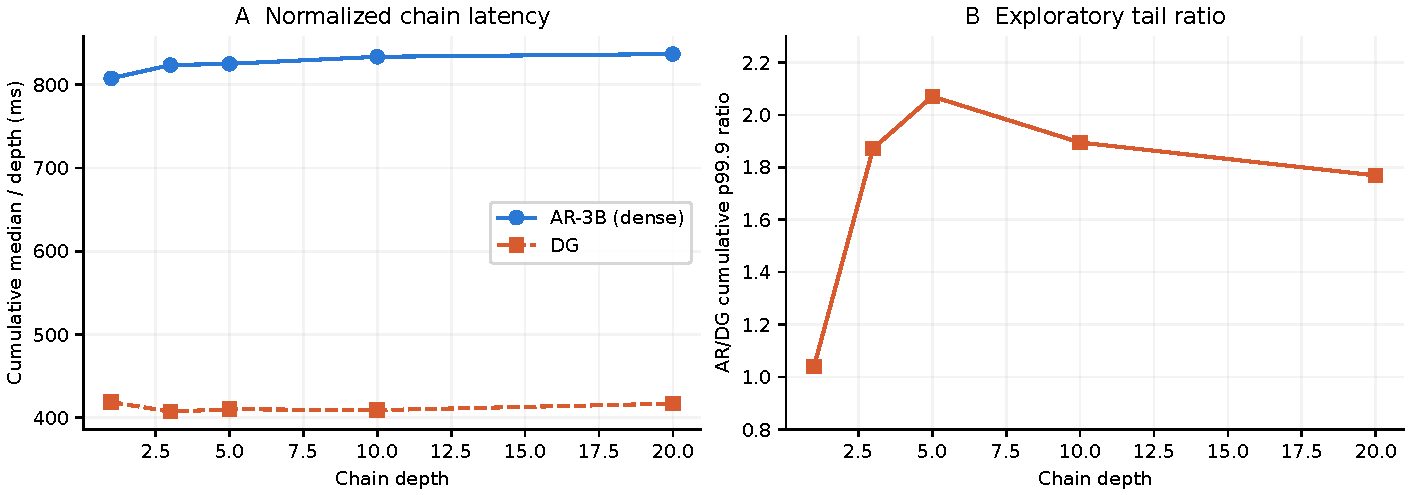
\includegraphics[width=\linewidth]{figures/fig10_usecase_chains.pdf}
\caption{BGL chain-harness latency (DG versus dense AR-3B; $n{=}100$
chains per depth, $K{=}8$). Cumulative median cost divided by depth is approximately constant
in this experiment. The cumulative tail ratio varies with depth.
With only 100 chains, the plotted p99.9 is effectively an extreme-order
statistic and should not be used to certify a production tail target.}
\label{fig:chains}
\end{figure}

The latency gap accumulates when several dependent calls are required,
but neither the quality of a complete investigation nor independence of
hop latencies follows from this curve. The HumanEval correction-chain
artifact reports total-chain and first-round medians; those are not
per-round latency growth rates (Appendix~\ref{app:humaneval}).

\paragraph{Reducing effort before a deadline.}
DG exposes a denoising-effort control, $K$. In the BGL sweep, reducing
$K$ from 8 to 4 lowers quality from \kEightFone{} to \kFourFone{}
while yielding p99 \kFourPninetynine\,ms. This operating point
falls below a 400\,ms service-time budget in that sample. It does not
guarantee valid JSON, completion under arbitrary interruption, or a
400\,ms end-to-end deadline. Selecting a lower $K$ before generation
is different from safely preempting an unfinished canvas.

Under an output-length cap of 128 tokens, DG's schema validity falls to
\dgValidTwentyEight\%, compared with \arValidTwentyEight\% for
dense AR-3B. Thus lowering denoising effort and shortening the output
budget have different effects (Appendix~\ref{app:quality}). AR also
admits adaptive budgets, early stopping, retries, and routing policies;
we do not claim that adaptive computation is unique to diffusion.
Grammar-constrained AR remains an important unmeasured comparator.

\paragraph{Wide schemas.}
Across schemas with 12--100 fields, DG's measured latency advantage
against dense AR-3B ranges from approximately $1.8\times$ to
$3.0\times$. Both prompt and output lengths change, and the models
emit different token counts. This is a useful workload comparison,
but does not isolate a benefit from joint inter-field reasoning.
The consistency evaluator checks three fixed rules over four fields at
every width, so it cannot establish scaling with the number of
pairwise constraints.

\begin{figure}[ht!]
\centering
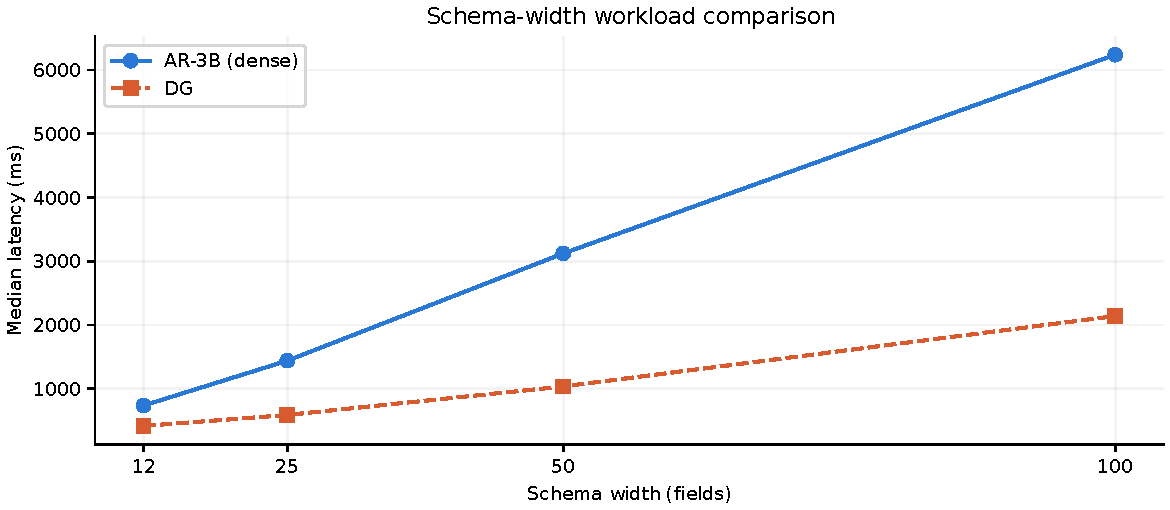
\includegraphics[width=0.85\linewidth]{figures/fig11_usecase_schema.pdf}
\caption{Latency versus schema width (BGL, $n{=}200$; dense AR-3B
baseline). DG's advantage rises from about $1.8\times$ to
$2.9$--$3.0\times$. Input length, output length, and canvas count
change together, preventing a causal attribution to schema width alone.}
\label{fig:schema}
\end{figure}

\paragraph{Adaptive effort: a measured negative result.}
A two-stage cascade first runs DG at $K{=}2$, checks structural-field
completeness, and reruns unresolved inputs at $K{=}8$. In the BGL
experiment ($n{=}200$), 29.5\% of records finish at the first stage
and 70.5\% escalate. F1 is 0.848 versus 0.853 for fixed $K{=}8$;
mean latency increases to 465\,ms from 376\,ms. The extra low-effort
pass costs more than it saves. Completeness is also only a proxy for
correctness. A lower escalation rate could improve this tradeoff, but
that benefit is not observed here.

\paragraph{Scope of application claims.}
The evidence concerns log extraction and exploratory code-generation
harnesses. We have not evaluated driving, trading, or deployed security
response, and do not infer suitability for those applications from
batch size or latency shape. Even in logs, the deployment choice depends
on quality, output validity, arrival rate, and the available AR baseline.
Appendix~\ref{app:refuted} reports the hypotheses that were contradicted
or left unsupported by the experiments.
